\section{POI, Query and Transition}
\label{sec:method}

\begin{figure}[t]
%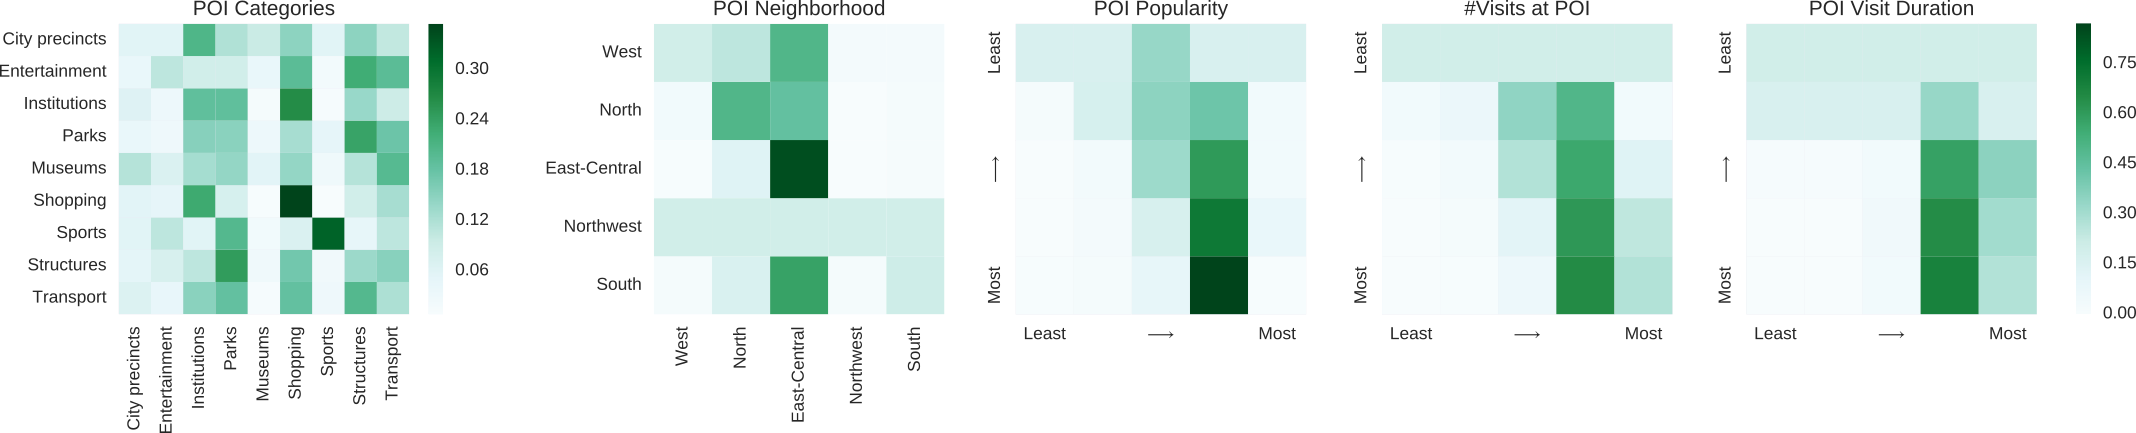
\includegraphics[width=\textwidth]{fig/poi_transmat.png}
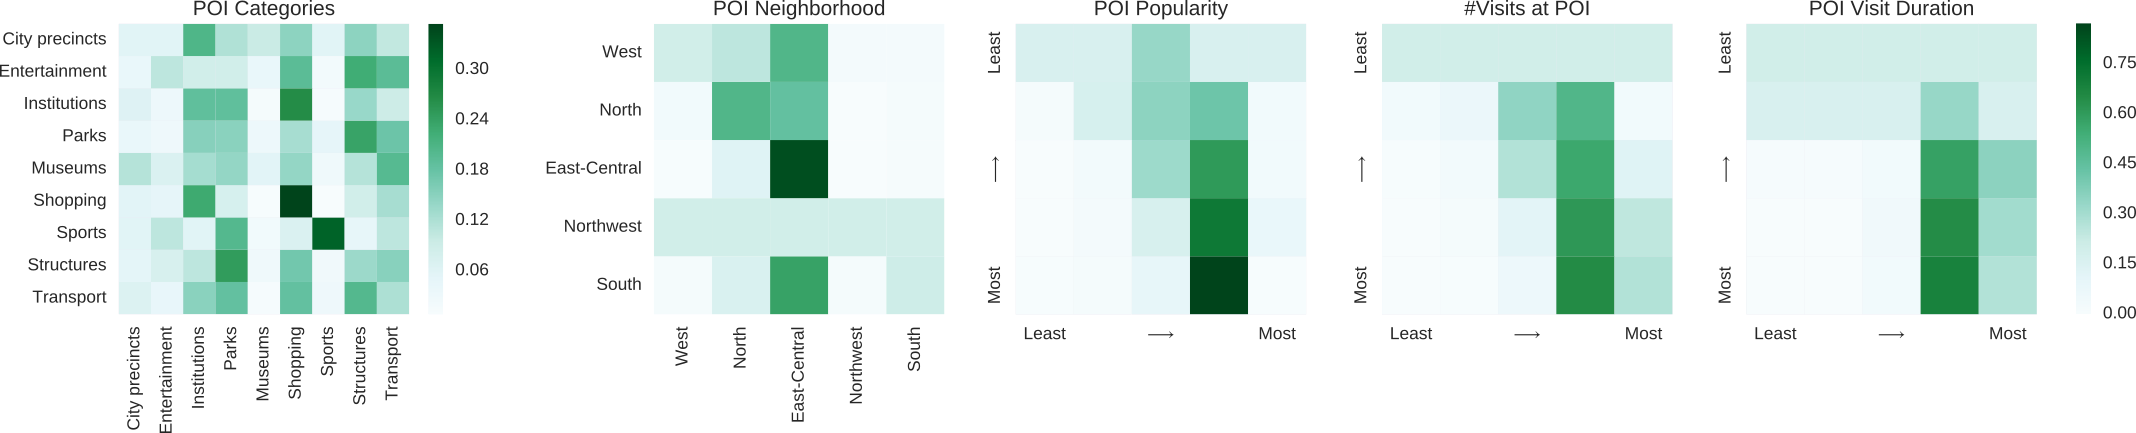
\includegraphics[width=\columnwidth]{fig/poi_transmat.png}
\caption{Transition matrices for five POI features: POI categories, neighborhood, popularity, number of visits, and visit duration. These statistics are from the Melbourne dataset. See Section~\ref{sec:transition} for descriptions.}
\label{fig:transmat}
\end{figure}


We aim to recommend a particular tour such that the user will visit a sequence of points-of-interests (POIs), denoted $p_1, \ldots, p_L$, that maximises utility. We are given the desired start ($p_1=p_s$) and end point ($p_L=p_e$), and an associated number $L$ of POIs desired, from which we propose a trajectory through the city. In Figure~\ref{fig:threesettings}(c), an example tour is shown in blue, which starts at the POI denoted as a grey star, visits two intermediate POIs, and terminates on the fourth POI denoted as a flag. The tour of length 4 can be modelled as a sequence of directed edges in a graph containing POIs in the city as nodes.

The training data consists of a set of tours of varying length in a particular city. We assume that all POIs $\mathcal{P}$ in the city are visited at least once by some user, and hence can construct a graph with POIs as nodes and potentially multiple directed edges between each pair of nodes. We extract the category, popularity, total number of visits and average visit duration for each POI.
%The set of categories are shown in Figure~\ref{fig:poicats} in the appendix, and the popularity is defined as the number of distinct users that visited the POI\cite{ht10}.



\subsection{POI Features and Query}
\label{sec:poifeature}

A naive approach would be to recommend the trajectory based on the popularity (number of distinct visitors)~\cite{ht10} of POIs only,
that is we always suggest the top-$k$ most popular POIs for all visitors given the start and end location, 
and its only adaptation to a particular request is to adjust $k$ to match the desired length.
In addition to popularity, 
we can also rank the candidate POIs based on the other three POI specific features (category, total visits and average duration).
Furthermore, since we are constrained by the fact that trajectories have to be of length $L$ and start and end at certain points, we hope to improve the recommendation by using this information.
In other words, using the \textit{query} $(p_s, p_e, L)$ we can construct new features by contrasting candidate POIs with $p_s$ and $p_e$.

For each of the POI features (category, total visits and average duration),
we construct two new features by taking the difference of the feature in POI $p$ with $(p_s, p_e)$ respectively.
For the category, we set the feature to $1$ when their categories are the same and $-1$ otherwise.
For popularity, total visits and visit duration, we take the real valued difference.
The distance from POI $p$ to $p_s$ (and $p_e$) is computed using the Haversine formula~\cite{haversine}.
Lastly we also include the required length $L$ of the trajectory as a feature.



\subsection{Transition probabilities}
\label{sec:transition}

In addition to information about each individual POI, a tour recommendation system would benefit
from capturing the likelihood of transitioning between different POIs. One option would be to
directly model the probability of going from one POI to another, but this has several weaknesses:
Such a model would be unable to handle a new POI (one that has not yet been visited).
Furthermore, even if we restrict ourselves to known POIs, there may be many locations which
are rarely visited, leading to significant challenges in estimating the probabilities from
empirical data.

We model POI transitions using a Markov chain with discrete factored states.
One difficulty of estimating the Markov chain is data sparsity, 
i.e., not enough transitions have been observed between every pair of POIs. 
We factorised the transition probability from POI $p_i$ to POI $p_j$ %is  according to
as a product of transition probabilities between pairs of individual POI features.
%as described in Table~\ref{tab:featuretran}.
POIs are grouped into $5$ clusters using K-means according to their geographical locations
to reflect their neighbourhood relations.
We directly model the transition between the category and neighbourhood of each POI as the conditional probability.
The popularity, total number of visits and the average visit duration are discretised by binning
them uniformly into $5$ discrete intervals on the log scale.
Figure~\ref{fig:transmat} visualises the transition matrices for individual POI features in Melbourne.

We compute the transition probabilities of the above individual POI features
using maximum likelihood estimation,
i.e., counting the number of transitions for each pair of features then normalising each row,
taking care of zeros by adding a small number $\epsilon$
%\footnote{In our experiments, $\epsilon = 1$.}
to each count before normalisation,
which results in a transition matrix for each of the above POI features.
%
Assuming independence between these features,
the transition probability $P(p_j | p_i)$ from $p_i$ to $p_j$ can be defined as the product
of the transition probabilities of each individual feature (and appropriately normalised),
with two additional constraints.
First we disallow self transitions by setting the probability of ($p_i$ to $p_i$) to zero.
Second we need to deal with the possibility that multiple POIs may share exactly the same feature vector.
When a group of POIs have identical (discretised) features, we distribute the probability uniformly among the POIs in the group. 
%More details of this procedure are provided in the Appendix.
The POI-POI transition matrix can be efficiently computed by taking the Kronecker product of
the transition matrices for the individual features and then updating it based on the constraints described above.
